%; whizzy chapter
% -initex iniptex -latex platex -format platex -bibtex jbibtex -fmt fmt
% 以上 whizzytex を使用する場合の設定。

%     Kansai Debian Meeting resources
%     Copyright (C) 2007 Takaya Yamashita
%     Thank you for Tokyo Debian Meeting resources

%     This program is free software; you can redistribute it and/or modify
%     it under the terms of the GNU General Public License as published by
%     the Free Software Foundation; either version 2 of the License, or
%     (at your option) any later version.

%     This program is distributed in the hope that it will be useful,
%     but WITHOUT ANY WARRANTY; without even the implied warranty of
%     MERCHANTABILITY or FITNESS FOR A PARTICULAR PURPOSE.  See the
%     GNU General Public License for more details.

%     You should have received a copy of the GNU General Public License
%     along with this program; if not, write to the Free Software
%     Foundation, Inc., 51 Franklin St, Fifth Floor, Boston, MA  02110-1301 USA

%  preview (shell-command (concat "evince " (replace-regexp-in-string "tex$" "pdf"(buffer-file-name)) "&"))
% 画像ファイルを処理するためにはebbを利用してboundingboxを作成。
%(shell-command "cd image200708; ebb *.png")

%%ここからヘッダ開始。

\documentclass[mingoth,a4paper]{jsarticle}
\usepackage{kansaimonthlyreport}
\usepackage[dvips]{xy}
\usepackage{ascmac}

% 日付を定義する、毎月変わります。
\newcommand{\debmtgyear}{2010}
\newcommand{\debmtgdate}{25}
\newcommand{\debmtgmonth}{04}
\newcommand{\debmtgnumber}{34}

\begin{document}

\begin{titlepage}

% 毎月変更する部分、本文の末尾も修正することをわすれずに

 第\debmtgnumber{}回 関西 Debian 勉強会資料

\vspace{2cm}

\begin{center}
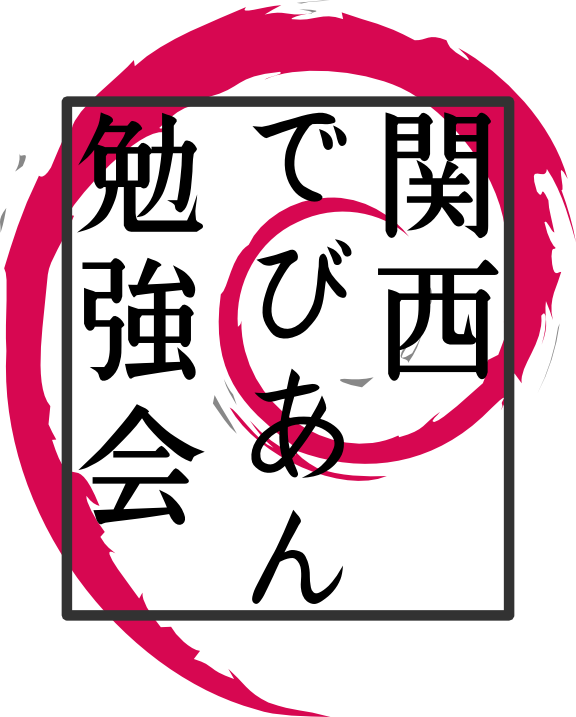
\includegraphics{image200802/kansaidebianlogo.png}
\end{center}

\begin{flushright}
\hfill{}関西 Debian 勉強会担当者 佐々木・倉敷・のがた \\
\hfill{}\debmtgyear{}年\debmtgmonth{}月\debmtgdate{}日
\end{flushright}

\thispagestyle{empty}
\end{titlepage}

\dancersection{Introduction}{Debian JP}

\subsection*{}%ロゴ用のスペース稼ぎ
 
関西 Debian 勉強会はDebian GNU/Linux のさまざまなトピック(新しいパッケー
ジ、Debian 特有の機能の仕組、Debian 界隈で起こった出来事、などなど)に
ついて話し合う会です。

目的として次の三つを考えています。
\begin{itemize}
      \item MLや掲示板ではなく、直接顔を合わせる事での情報交換の促進
      \item 定期的に集まれる場所
      \item 資料の作成
\end{itemize}

それでは、楽しい一時をお楽しみ下さい。

\clearpage

\begin{minipage}[b]{0.2\hsize}
 {\rotatebox{90}{\fontsize{80}{80}
{\gt 関西デビアン勉強会}}}
\end{minipage}
\begin{minipage}[b]{0.8\hsize}
\hrule
\vspace{2mm}
\hrule
\setcounter{tocdepth}{1}
\tableofcontents
\vspace{2mm}
\hrule
\end{minipage}

\dancersection{事前課題}{のがたじゅん}

2月から関西Debian勉強会でも事前課題を始めました。

2010年4月の事前課題は以下です。

\begin{enumerate}
 \item あなたのDebianデスクトップ環境について(どういうデスクトップ環境使っ
       ているのか、何か工夫をしているかなど)教えてください。Debianデスク
       トップ環境を使っていない人は、なぜ使っていないのか教えてください。
 \item /etc/passwdを解析して、ユーザbinのログインシェルを表示するできるだ
       けシンプルな方法(プログラム/スクリプト/コマンドライン)を考えな
       さい。
\end{enumerate}

申し込みをされた方の回答は以下になります。

\begin{prework}{ 白方 健太郎 }

 \begin{enumerate}
  \item サーバーでしか使ってないのでデスクトップ環境ありません…。
  \item  
\begin{commandline}
    perl -n -e 'if(/^bin:.*:.*:.*:.*:(.*)/){print $1;}' /etc/passwd
\end{commandline}

\end{enumerate}

\end{prework}

\begin{prework}{ かわだ }

\begin{enumerate}
 \item デスクトップ環境
\begin{itemize}
      \item   GNOME
      \item インストール時にデフォルトで入れてほぼそのままです。
\end{itemize}
  \item  
\begin{commandline}
    sed -n "s/^bin:.*:\([^:]\{1,\}\)$/\1/p" /etc/passwd
    grep ^bin: /etc/passwd|cut -f7 -d:
\end{commandline}
\end{enumerate}
\end{prework}

\begin{prework}{ IPv6waterstar }

 \begin{enumerate}
       \item ノーマルかCompizを使ったりします。
       \item 日曜日までに考えます。
 \end{enumerate}
\end{prework}
\begin{prework}{ say.no00 }
    \begin{enumerate}
          \item KDE
        \begin{itemize}
              \item
            GNOMEが多かったのでちょっと違ったのが使いたかったのと、GIS関係がQtを利用しているものが多いので、親和性が高そうだったから。
        \end{itemize}
          \item すいません、時間がなくて解析出来ていません。当日までに時間ができたらトライしておきます。
    \end{enumerate}
\end{prework}
\begin{prework}{ dictoss(杉本 典充) }
 \begin{enumerate}
       \item ある程度のパワーがあるマシンの場合はXfce4、パワーがないマシンの場合はIceWMを使用します。

選ぶ基準は、軽いこと、ランチャーが使いやすいこと。(無線LANのランチャーがあると便利) Ctrl+Escコマンドでメニュー表示、Alt+Tabでのウィンドウ切り替えは便利です。画面いっぱいに1つ、2つ、3つのターミナルを同時に起動する小さなスクリプトを使用しており、複数のターミナルを使う作業が楽になります。
  \item  
     \begin{commandline}
         grep ^bin: /etc/passwd | tr ':' '\n' | tail -n 1
     \end{commandline}
\end{enumerate}

\end{prework}

\begin{prework}{ 佐藤誠 }
\begin{enumerate}
 \item (回答なし)
 \item  
\begin{commandline}
    $ sed -n '/^bin:/s@[^:]*:@@gp' /etc/passwd
\end{commandline}
\end{enumerate}
\end{prework}

\begin{prework}{ 山下康成@京都府向日市 }
\begin{enumerate}
 \item Debianデスクトップ環境は使ってません。
昔々、Debian 1.x だったか 2.x だったかをインストールする時、dselectか何かで一つ一つのパッケージをインストールするか否かを指定させられ、Debianを挫折しました。それ以来Debianデスクトップ環境は使ってません。必要に迫られてサーバ環境でのみ使わせていただいています。
 \item 模範解答(?)はセッション資料をご覧下さい。
\end{enumerate}
\end{prework}

\begin{prework}{ ”まさ”こと”甲斐正三”です }
\begin{enumerate}
      \item わたしのDebianデスクトップ環境:
    Debianデフォールトのgnome desktopを使っています。
    上パネルには、”ワークスペース切り替え噐”、”画面のロック”
    ”gnome目玉”を、下パネルには、”システムモニター”、
    ”お天気gnome”を配置しています。
 \item 
\begin{commandline}
     #! /usr/bin/python2.5
    import commands, string
    a = commands.getoutput('whoami')
    b = 'grep ' + a + ' /etc/passwd')
    c = commands.getoutput(b)
    d = c.split(':')
    e = d[len(d)-1]
    print e 
    #  動作確認はしておりません
\end{commandline}
\end{enumerate}

\end{prework}

\begin{prework}{ 佐々木洋平 }

\begin{enumerate}
 \item Desktop:
       \begin{itemize}
             \item WindowMaker のキーバインドにどっぷりつかってしまったので、
           未だに WindowMaker のキーバインドから離れられません.
           軽くて見栄えの良い WindowManager が好きです. Gnome やKDE はリソースの管理をどこでやっているのか追跡するのを諦めた時点で使うのを止めました(Gnome だと gconf? kde だと何?)
             \item 
           現在は XFce4 を使用しています。とは言っても XFce4 らしさは
           まったく無いですね.
           偶にXFce4 + Compiz-Fusion も使ってます. とは言ってもCompizらしさは(ry. 基本「エクスポーズ」が使いたいだけだったので、最近は Compiz-Fusion も触ってません.
        \item LXDE も試してみましたが WindowMaker 風のキーバインドへカスタマイズできなくて断念しました.
       \end{itemize}
 \item
普段なら[1]ですが bash だけでやるなら、例えば[2]とかですか?(古い bash だと動きませんが)
       \begin{commandline}
        [1]$ grep -e "^bin" /etc/passwd | cut -d 7 -S:
        [2]$ while read l; do [[ $l =~ ^bin ]] && echo ${l##*:}; done < /etc/passwd
       \end{commandline}
       
\end{enumerate}
\end{prework}


\begin{prework}{ hajime.mizuno }

\begin{enumerate}
 \item Ubuntuっていう最新のDebianを使ってマス。……というのは冗談で、
 Ubuntuでバグっぽいものを踏んだ際にDebianの挙動やパッケージバージョンを確
 認するため、Sidを使っています。ぶっちゃけ端末とEmacsがあればいいので、デ
 スクトップとしての工夫はないかも。
 \item 
\begin{commandline}
    $ egrep '^bin:' /etc/passwd | cut -d : -f 7
\end{commandline}

\end{enumerate}

\end{prework}

\begin{prework}{ 山田 洋平 }
\begin{enumerate}
 \item Debianデスクトップ環境:使っていません。(使いこなせない。)他のパッケージと機能が被っているから、かな...必要を感じないです。
 \item /etc/passwd の解析:passwd はコロン区切りなので awk を使うと簡単[1]、でも正規表現がテーマなら sed を使った方法[2]も書いておきます。同じことを拙い perl で書けば[3]。
\begin{commandline}
    [1] $ awk -F: '$1=="bin"{print $NF}' /etc/passwd
    [2] $ sed -n '/^bin:/s/.*://p' /etc/passwd
    [3] $ perl -ne '/^bin:/ and s/.*:// and print' /etc/passwd
\end{commandline}
\end{enumerate}
\end{prework}

\begin{prework}{ のがたじゅん }
 \begin{enumerate}
       \item デスクトップ環境はノートはKDE 4.4、デスクトップはLXDEを使っていま
     す。それ以外にはキーボードランチャーのGnome DoのDockyは必須です。
     その他、音関係をPulseAudioにしたり、ネットワークの管理をWicdにし
     たり、かっこいいスプラッシュ画面を妄想しています。
       \item  
     \begin{commandline}
         $ grep ^bin /etc/passwd | cut -d':' -f 7
     \end{commandline}
 \end{enumerate}
\end{prework}

\dancersection{最近のDebian関係のイベント報告}{Debian JP}

\subsection{前回の関西Debian勉強会}

\begin{wrapfigure}{r}{5.5cm}
 \begin{center}
 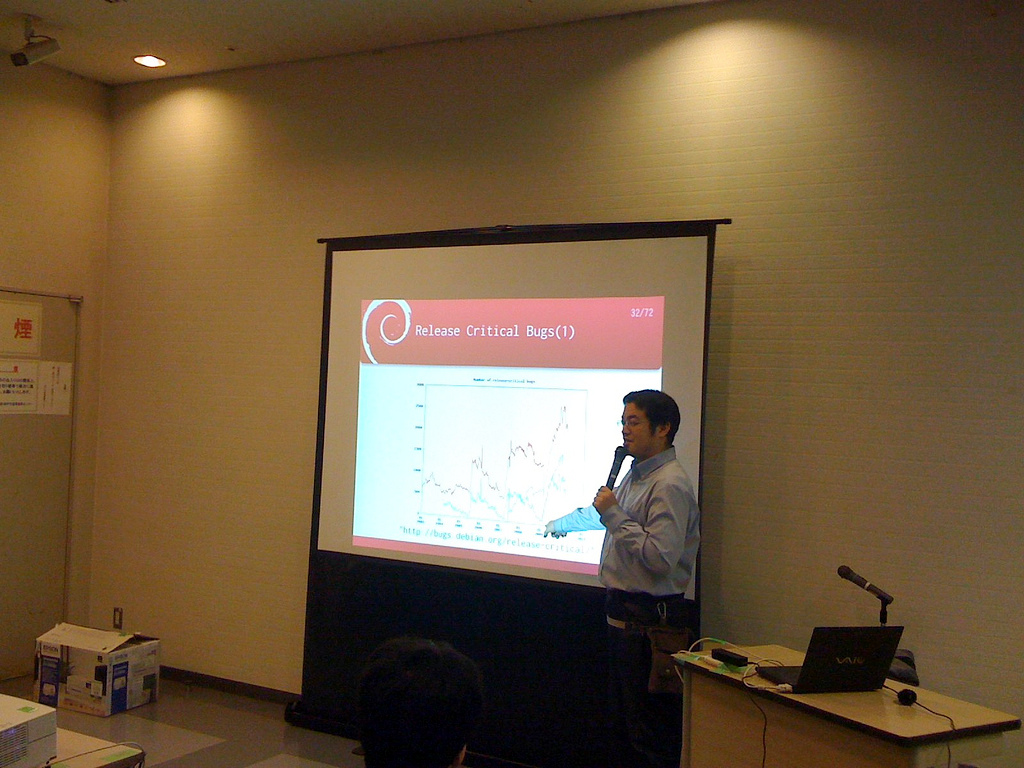
\includegraphics[width=5cm]{image201004/osckobe.jpg}
 \caption{オープンソースカンファレンスKobeでのセッション}
 \end{center}
\end{wrapfigure}

前回の関西Debian勉強会は、3月13日神戸市産業振興センターで開催されたオープ
ンソースカンファレンス 2010 Kansai@Kobeのセッションとしておこなわれまし
た。

セッションは佐々木洋平さんから「Squeeze off! 次期リリース Debian 6.0
Squeezeを見てみよう」というタイトルで、Debianの次期リリースSqueezeについ
ての概要と、今、リリースに必要とされる作業について発表されました。

会場がオープンスペースということもあり気軽に参加された方も多く、基本的な
Debianのリリースについてなど、活発な質問のやりとりがおこなわれました。


\subsection{第63回 東京エリア Debian 勉強会}

先週土曜日 4 月 17 日には東京エリア Debian 勉強会が開催されました。
\begin{description}
      \item[piuparts] 
    パッケージのインストール/アップグレードのテスト環境
      \item[upstarts]
    イベントドリブンな init
      \item[debtags]
    パッケージに付与されたタグを元に簡便に検索するツール
\end{description}
について熱い議論がなされた模様です。


\subsection{2010年度Debian開発者の会役員選挙とDebian Project Leader選挙}
Debian JP Project役員任期終了に伴う役員改選選挙が開催され、
会長に荒木靖宏さん、監事に山下尊也さんが選出されました。

また、Debian ProjectではDebian Project Leaderの選挙がおこなわれ、投票の結
果、Stefano Zacchiroliさんが選出されました。
Debian Project Leader選挙の詳しい結果については、
\url{http://www.debian.org/vote/2010/vote_001}をご覧ください。

\subsection{snapshot.debian.orgの運用が始まりました}
日々更新されるDebianパッケージを保存する
\url{http://snapshot.debian.org/}の運用が始まりました。

アーカイブされるパッケージは2005年3月以降のdebian、debian-securityと、
debian-volatile、backports.org、debian-archive、debian-portsのほぼすべて
のパッケージです。

Sidを使っている人にとっては、とても心強いですね。


\subsection{freeze 延期}

既にご存知かと思われますが、
ftp master のハードウェアトラブルなどの要因から、
3 月末に予定されていた squeeze の freeze は 5 月末〜6月上旬に延期になりました。

というわけで、リリースに向けた Bug Squash や翻訳はまだまだ間に合います。 皆さん頑張りましょう!



\dancersection{みんなのDebianデスクトップ環境を見てみよう}{佐々木洋平、
のがたじゅん}

\subsection{はじめに}
春です。就職や進学で新しい環境になり、新たにDebianをインストールして使い
始めた方も多いでしょう。
そこで、Debianをデスクトップ環境で使っている人の環境を見ながら、Debianデ
スクトップ環境について考えてみたいと思います。

\subsubsection{Debianリファレンスを読もう}
Debianを使い始める前に、青木 修さんが日本語に翻訳された「Debianリファレン
ス」(\url{http://www.debian.org/doc/manuals/reference/})を読んみましょう。
デスクトップ環境については、第7章の「X Windowシステム」は多くのヒントがあると思うので、きっと役に立つと思います。

\subsubsection{Debianデスクトップ環境インストールTips}
Debianの標準デスクトップ環境はGNOMEと思われていますが、Debian
Installer(d-i)に

\begin{commandline}
 desktop=gnome|kde|xfce|lxde
\end{commandline}

と、オプションをつけてtaskselに「デスクトップ環境」を指定すると、それぞれ
のデスクトップ環境がインストールされます。

\subsubsection{統合デスクトップ環境とウィンドウマネージャの違い}

Debian(を含めた unix 環境)に初めて触れる方にとって「統合デスクトップ環境とウィンドウマネージャの違い」と言われても「なに?」と思われる方もいらっしゃるでしょう。

統合デスクトップ環境とは、GNOMEやKDEなどのようにアイコンやタスクバーがあり、ファイルマネージャなどを使ってグラフィカルにファイル操作などができる環境をいいます。

もう一つのウィンドウマネージャについてですが、こちらは統合デスクトップ環境からグッと範囲が狭くなり、X.orgなどのウィンドウシステムで、ウィンドウの配置や外観、そのウィンドウへの入力(フォーカス)を管理するソフトです。乱暴ですが「ウィンドウの枠」と言えばわかりやすいかもしれません。

ウィンドウマネージャには、ウィンドウを重ね合わせて表示するスタックな形のウィンドウマネージャのほかに、画面全体を使いウィンドウをタイルのように敷き詰めて利用する、タイル型ウィンドウマネージャもあります。\footnote{%
日本タイル型ウィンドウマネージャ推進委員会 Wiki -SourceForge.JP:\\
\url{http://sourceforge.jp/projects/tilingwm/wiki/FrontPage}}

\subsection{統合デスクトップ環境あれこれ}

\subsubsection{Gnome - GNU Network Object Model Environment}
\begin{wrapfigure}{l}{5.5cm}
 \begin{center}
  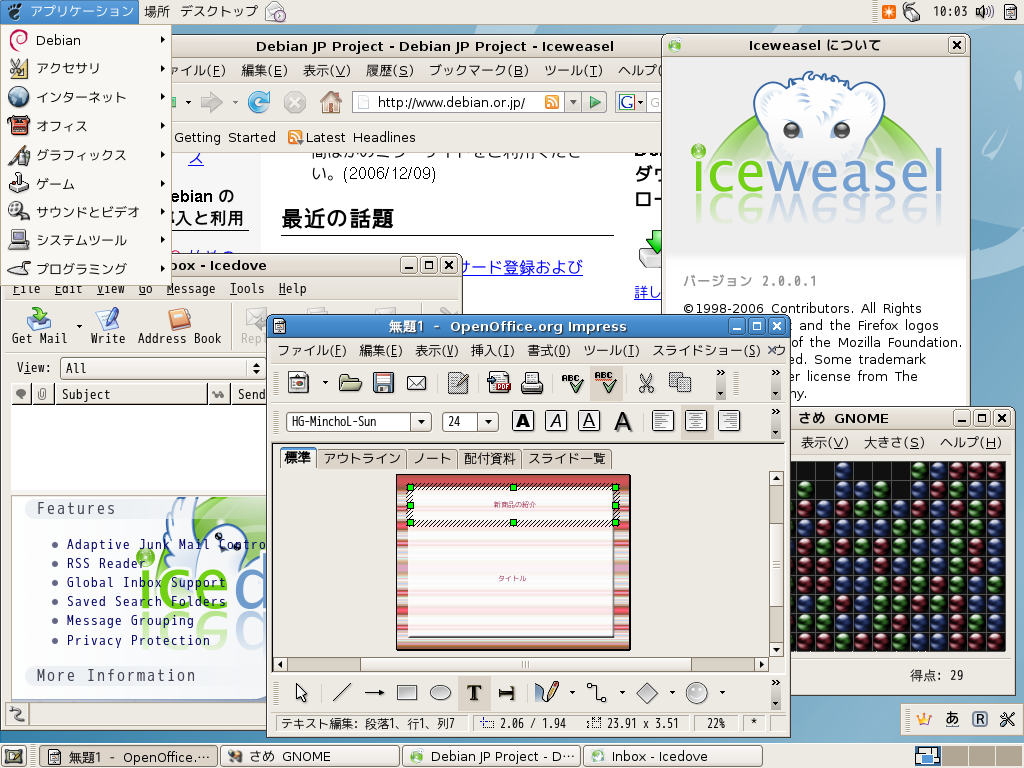
\includegraphics[width=5cm]{image201004/gnome.png}
  \caption{lenny での Gnome の画面}
 \end{center}
\end{wrapfigure}


GNOME は GUI ツールキットに GTK+ を使用した統合デスクトップ環境です。
Lenny に収録されているのは 2.22、
現在 squeeze に収録されているのは 2.28 です。
最新版は 2.30 ですが、これが squeeze に入るかは未だわかりません。

Linux において「統合デスクトップ環境」という単語が目立ち始めた時から KDE(後述)と双璧をなして発展してきました。
現在では「統合デスクトップ環境」と言えば、この GNOME か KDE(後述)と言って良いくらい流行っています。
Debian ではインストーラで GUI インストールを選択すると GNOME のデスクトップ環境が導入されます。
また、Ubuntu でも標準で採用されているため馴染のある人も多いかもしれません。

\vspace{1em}

GNOME をインストールするには、
タスクから「Gnome デスクトップ環境」を選ぶか、導入したいパッケージの量に合わせて
\begin{description}
      \item[gnome] 
    GNOME 環境全て(GNOME プロジェクトが配布していない物も含める)
      \item[gnome-desktop-enviornment]
    GNOME プロジェクトの公式配布物としてのGNOME 関連のパッケージ全て
      \item[gnome-accessibility]
    必要最小限のパッケージにスクリーンリーダなどの小物を加えた環境
      \item[gnome-core]
    必要最小限の環境。アプリケーションは別途導入する必要がある
\end{description}
等のメタパッケージをインストールします。

その他、DebianでのGNOMEについては、Debian GNOME Packaging に情報が集まっているので参考にするとよいでしょう。

\begin{itemize}
 \item Debian GNOME Packaging

       \url{http://pkg-gnome.alioth.debian.org/}

\end{itemize}


\subsubsection{KDE -- the K Desktop Environment}
\begin{wrapfigure}{r}{5.5cm}
 \begin{center}
  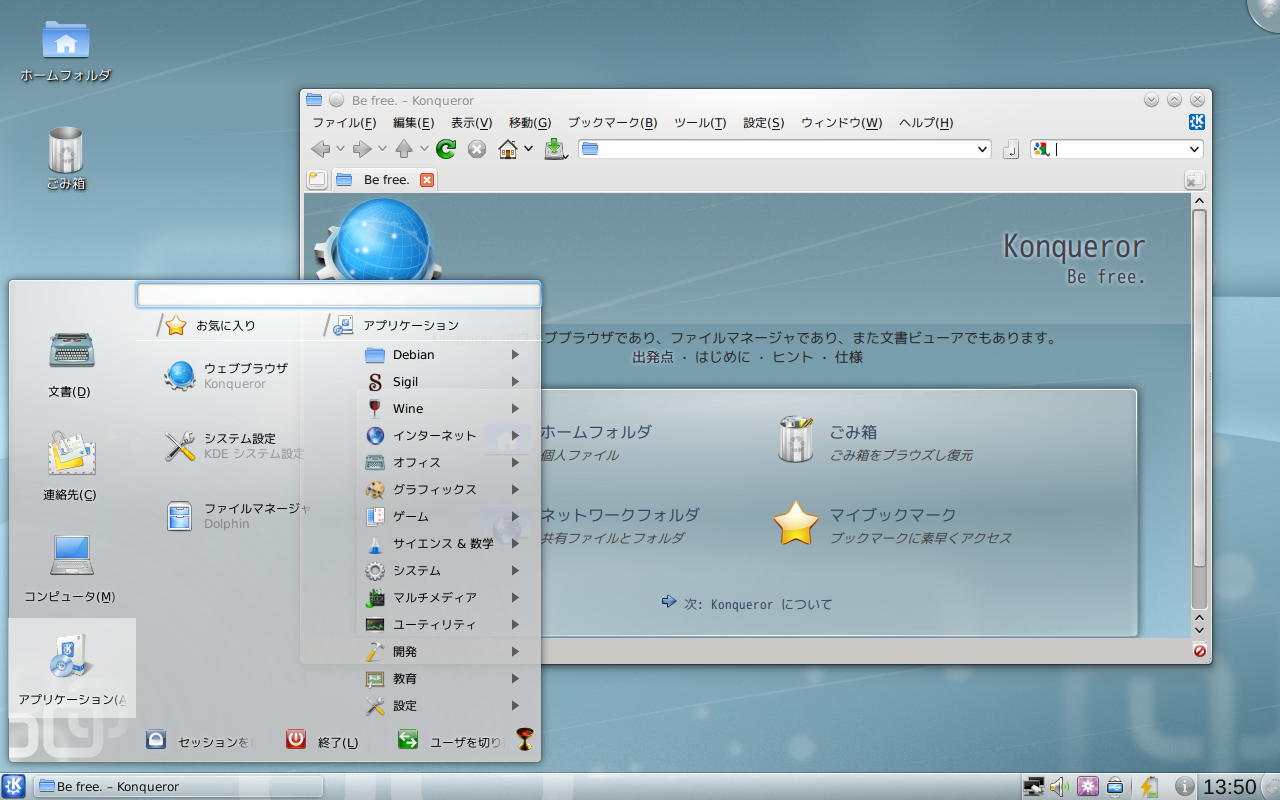
\includegraphics[width=5cm]{image201004/kde44.png}
  \caption{KDE 4.4の画面}
 \end{center}
\end{wrapfigure}

KDEは、GUIツールキットにQt(キュート)を利用した統合デスクトップ環境で、
LennyではリリースのタイミングからKDE 3.5、Squeeze/SidではKDE 4.3、
ExperimentalにはKDE 4.4が収録されています。(2010年4月現在)

KDE 3系とKDE 4系は、ツールキットがQt3とQt4が違うほか、機能やデスクトップ
自体の考え方まで変わっているのでKDE 3系が好きだった人はとまどうかもしれま
せん。

KDEをインストールするには、タスクから「KDE デスクトップ環境」を選ぶか、
導入したいパッケージの量に合わせて
\begin{description}
      \item[kde]
    KDE 環境全て(KDE プロジェクトが配布していない物も含める)
      \item[kde-core]
    必要最小限の環境。アプリケーションは別途導入する必要がある
\end{description}
等のメタパッケージをインストールします。

その他、DebianでのKDEについては、Debian KDE Maintainersのサイトに情報が集
まっているので参考にするとよいでしょう。

\begin{itemize}
 \item The Debian KDE maintainers website:

       \url{http://pkg-kde.alioth.debian.org/}

\end{itemize}

\subsubsection{Xfce4}
\begin{wrapfigure}{r}{5.5cm}
 \begin{center}
  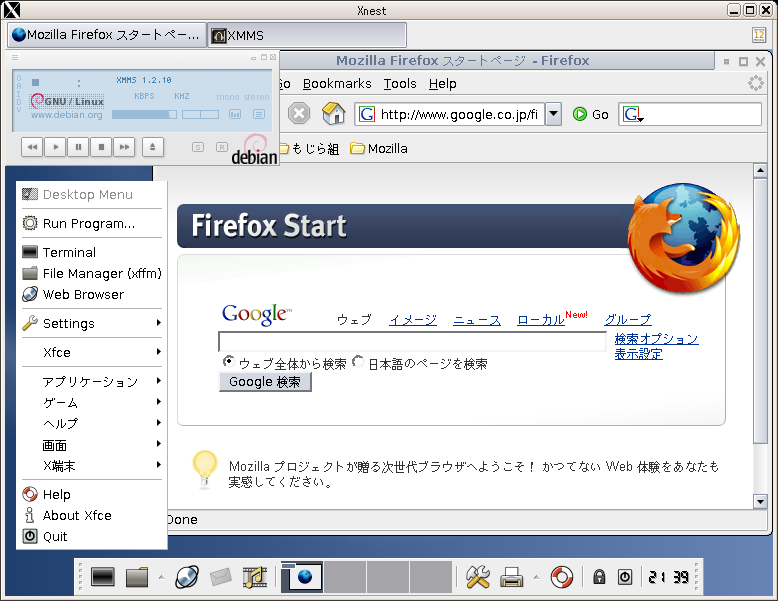
\includegraphics[width=5cm]{image201004/xfce4.png}
  \caption{Xfce4 の画面}
 \end{center}
\end{wrapfigure}


GNOME や KDE はそれなりにメモリを喰いますし、それなりに重いです。
そこで X で利用できる軽量なデスクトップ環境の構築を目標として作成されたのが
Xfce です。名前の由来は {\it XForms Common Environment} です。
ver.3 までは GUI ツールキットとして XForms を使用し、商用 UNIX の CDE(Common Desktop Environment)を模していましたが、
ver.4 以降はGUI ツールキットとして GTK+2 を使用し、
それまでと雰囲気ががらりと変わりました(そんな訳で ver.4 以降を強調するために Xfce{\bf 4} と呼ぶ事も多いです) 。

同じ GTK+ を使用している Gnome と比較して(見た目も綺麗な割に)非常に軽量に動作するのが特徴です。また、プロジェクトの公式配布物ではないものの、Xfce Goodies と呼ばれるプラグインが続々と開発されており、非常に使い易い環境となっています。


Xfce4 をインストールするには、タスクから「Xfce デスクトップ環境」を選ぶか、
{\tt xfce4} パッケージおよび {\tt xfce4-goodies}パッケージをインストールします。


その他、Debianにおける Xfce に関する情報は Debian Xfce Group のサイトに情報が集
まっているので参考にするとよいでしょう。

\begin{itemize}
 \item Debian Xfce Group:

       \url{http://pkg-xfce.alioth.debian.org/}

\end{itemize}



\subsubsection{LXDE}
\begin{wrapfigure}{l}{5.5cm}
 \begin{center}
  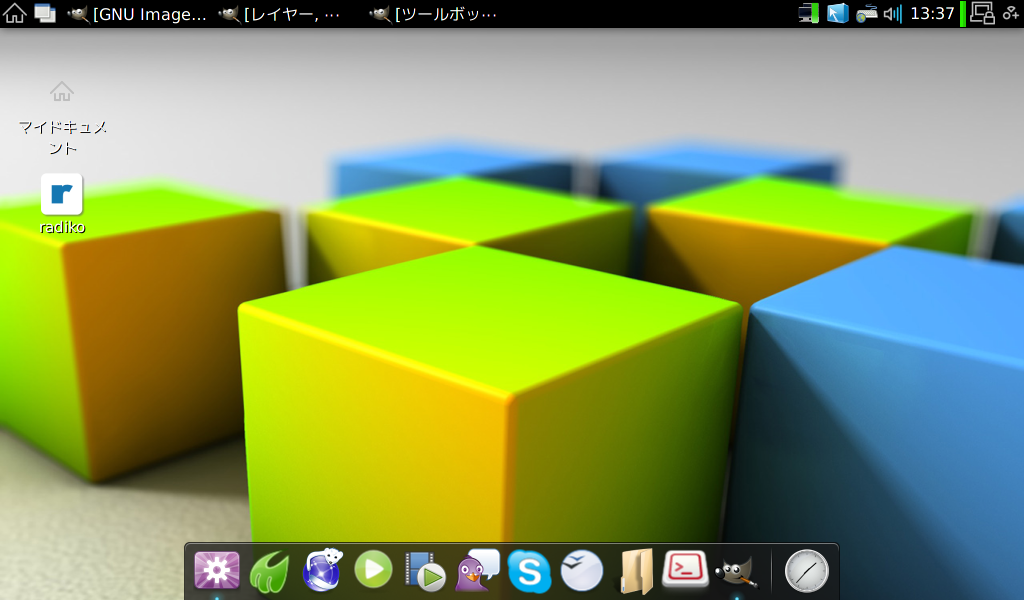
\includegraphics[width=5cm]{image201004/lxde-eeepc.png}
  \caption{LXDEをeeePCで利用している画面(ランチャーはGNOME Do)}
 \end{center}
\end{wrapfigure}

LXDEは初期起動時のメモリ使用量が100MBほどの軽量なデスクトップ環境です。

LXDEはGNOMEやKDE、Xfce4などの他のデスクトップ環境と比較すると、統合デスク
トップ環境としての共通ライブラリなどがなく、ウィンドウマネージャに
OpenBox、ファイルマネージャにPCManFM、パネルにlxpanelなど軽量のアプリケー
ションを組み合わせ、ゆるやかな形として統合デスクトップ環境を実現していま
す。

DebianでのLXDEパッケージはAndrew Leeさんが管理しています。

インストールについてはKDEと同様、lxdeというメタパッケージが用意されている
ので、aptitudeでサクっとインストールできます。
\\
\begin{commandline}
$ sudo aptitude install lxde
\end{commandline}

SqueezeのLXDEについてですが、何が原因でブロックされているのか少しよく分か
らないのですが、0.4.2の中途半端な形で止まっていてインストールしても使うこ
とができません。GDMからログインすると強制的にログアウトさせられるし、startxで起動すると Segmentation Faultするし、これはちょっと深刻なのでこの辺ことをを知ってる人がいたら教えてください。RCバグで登録されてる「\#575972 - lxappearance: segmentation fault on trying to change themes \url{http://bugs.debian.org/cgi-bin/bugreport.cgi?bug=575972}」とも違うっぽいです。


\dancersection{ハッカーに一歩近づく Tips 〜正規表現編〜}{山下康成@京都府向日市}

\subsection{正規表現とは}

検索や置換などテキスト処理で使用する効率的なパターンマッチングの表現方法。
ファイル名に使う *, ? と概念は同じ。 
今回、説明するのは

\begin{commandline}
^$.[]*¥(){}    
\end{commandline}
のたった11文字+数字

\subsection{事前課題}

/etc/passwd を解析してユーザ binのログインシェルを表示しなさい
\begin{enumerate}
      \item 思考に近い解答例
    \begin{commandline}
        % grep '^bin:' /etc/passwd|cut -d: -f7  
    \end{commandline}
      \item 空気を読んで正規表現を使った解答
    \begin{commandline}
        % sed -n -e 's/^bin:.*:¥([^:]*¥)$/¥1/p' /etc/passwd        
    \end{commandline}
\end{enumerate}

\subsection{正規表現で使う文字}
\subsubsection{ \^ ~と \$}
\begin{description}
      \item[{\tt \^}] 行頭に一致
      \item[{\tt \$}] 行末に一致
\end{description}
行頭(\^ ), 行末(\$ )にマッチさせる場合の例:
\begin{commandline}
      % grep '^bin:' /etc/passwd
      % grep '/bash$' /etc/passwd 
\end{commandline}
grep 以外でも、emacs や vi でも同じ様に使える。もちろん, perl や awk でも...
\begin{commandline}
    emacs   ->  RE search: ^bin
    vi      ->  /bash$
\end{commandline}

\subsubsection{{\tt .} ピリオド}

何か一文字に一致する。
文字数だけが一致すれば良いときや
何か文字があることが重要なときに使う

\subsubsection{列挙}

列挙したどれかに一致させたいとき。
例: bin や root など b, r で始まるユーザを表示
\begin{commandline}
          % grep '^[br]' /etc/passwd
\end{commandline}
ほかには
\begin{commandline}
        [! " \# ]  !, ", \# に一致
        [0-9]  半角数字1文字に一致
        [A-Za-z]  英字に一致
\end{commandline}

\subsubsection{[\^~列挙]}

列挙したどれにも一致させたくないとき。
例: daemon や sys など b, r 以外で始まるユーザを表示 
\begin{commandline}
    % grep '^[^br] /etc/passwd    
\end{commandline}
※行頭を表す \^~ と [~] 内の \^~ とは、同じ文字だが意味が違う

\subsection{*(アスタリスク)}

すぐ前の文字/正規表現0回以上に一致。
例:
\begin{commandline}
    何がいくつあっても一致
      .* 
    ホワイトスペースがいくつあっても一致
      [<space><tab>]* 
\end{commandline}

\subsubsection{¥{n,m¥}}

すぐ前の文字/正規表現n回以上m 回以下に一致。m は省略可能
\begin{commandline}
    ホワイトスペースが1個以上あれば一致
    [<space><tab>]¥{1,¥} 
    数字が1文字以上5文字以下(例えばざっと short の範囲)あれば一致
    [0-9]¥{1,5¥} 
\end{commandline}

\subsubsection{( ) と $\backslash$n}

( ) で囲んだところを順に $\backslash$1 ,$\backslash$2 ... として使える。
置換に使うと置換元の一部を使える。
vi の ex モードや、emacs の replace regexp でも使える。 
例:
\begin{commandline}
      # aaa bbb 等、行頭に同じ文字が3つある時に一致 
      % echo 'aaa' | grep '^¥(.¥)¥1¥1'
      # abab 1212 等、行頭から2文字の繰り返しに一致 
      % echo 'abab' | grep '^¥(.¥)¥(.¥)¥1¥2'
      % echo 'abcd' | sed - e 's/^¥(.¥)¥(.¥).*$/1文字目は ¥1、2文字目は ¥2 です/' 
\end{commandline}

\subsection{事前課題の空気を読んだ解答をレビュー}
\begin{commandline}
sed -n -e 's/^bin:.*:¥([^:]*¥)$/¥1/p' /etc/passwd
{
      行頭がbin:で
      何か文字が 0 文字以上あって
      : があって
      : 以外が 0 以上あるところを1番目のバッファにいれて
      行末
}
\end{commandline}
というパターンがあれば、1番目のバッファを表示する.

\subsection{実例}
\subsubsection{ssh アタッカーをブロックする}
/var/log/daemon.log に
\begin{commandline}
      Apr 11 04:46:07 ns sshd[31776]: Invalid user oracle from 211.233.73.66

      Apr 11 09:17:05 ns sshd[5607]: Did not receive identification string from 211.155.227.20
\end{commandline}
      のような行があれば、その IP アドレスを /etc/hosts.deny に登録する
      \begin{commandline}          
      #! /bin/sh
      # Apr 11 04:46:07 ns sshd[31776]: Invalid user oracle from 211.233.73.66
      # Apr 11 09:17:05 ns sshd[5607]: Did not receive identification string from 211.155.227.20 
      LANG=C
      export LANG

      HOSTSDENY=/etc/hosts.deny 
      sed -n ¥
      -e 's/^.* sshd.*: Invalid user .* from ¥([0-9][0-9¥.]*¥)/¥1/p' ¥
      -e 's/^.* sshd.*: Did not receive identification string from ¥([0-9][0-9¥.]*¥)/¥1/p' ¥
      /var/log/daemon.log | sort -u |
      while read IP
      do
      # /etc/hosts.deny
              
      L=`grep '^ALL : '$IP'$' $HOSTSDENY`
      
      if [ "$L" = "" ]
      then
      echo "ALL : $IP" >> $HOSTSDENY
      fi
      done
  \end{commandline}


\subsubsection{%
ロードアベレージが3以上なら、日時とps ax の結果を /tmp/highload に残す}
\begin{commandline}
      # LANG=C uptime
      11:57PM  up 165 days,  2:26,  1 user,  load average: 0.00, 0.06, 0.07
\end{commandline}
      のロードアベレージの一つ目を切り出す

      \begin{commandline}
      #! /bin/sh 
      LOAD=`LANG=C /usr/bin/uptime | sed -e 's/^.*: ¥([0-9]*¥)¥.[0-9]*,.*$/¥1/'
      if [ "$LOAD" -ge 3 ]
      then
            echo >> /tmp/highload
            date >> /tmp/highload
            ps ax >> /tmp/highload
      fi
      \end{commandline}


\subsubsection{キモ }

行頭もしくは行末を起点にパターンマッチをすると良い場合が多い。
\^~ と \$ とを活用。
スペース区切りは TAB とスペースがいくつあるかわからない。
\begin{commandline}
[<SP.><TAB>][<SP><TAB>]*
[<SP.><TAB>]¥{1,¥}
\end{commandline}

\subsection{おわりに}

正規表現をうまく使いこなせれば操作が少なくなり、
もしくはスクリプトが小さくできて効率的。 正規表現をマスタして、ハッカーに一歩近づこう!

\dancersection{今後の予定}{Debian JP}

\subsection{次回の関西Debian勉強会}
次回、2010年5月の関西Debian勉強会は 5月23日におこなう予定です。
Ubuntu Japanese Team のあわしろいくやさんをお招きして
リリースされた Ubuntu の最新 LTS について語って頂きます。
また関西Debianからは、きっとフリーズ間近の squeeze のお話をする予定です。

\subsection{オープンソースカンファレンス 2010 Kansai@Kyoto}
申し込みが始まりました。


% 冊子にするために、4の倍数にする必要がある。
% そのための調整
%\dancersection{メモ}{}
%\mbox{}\newpage

\printindex
 \cleartooddpage

 \begin{minipage}[b]{0.2\hsize}
  \rotatebox{90}{\fontsize{80}{80} {\gt 関西デビアン勉強会} }
 \end{minipage}
 \begin{minipage}[b]{0.8\hsize}

 \vspace*{15cm}
 \rule{\hsize}{1mm}
 \vspace{2mm}
 
\includegraphics[width=2cm]{image200502/openlogo-nd.eps}
 \noindent \Large \bf Debian 勉強会資料\\ \\
 \noindent \normalfont \debmtgyear{}年\debmtgmonth{}月\debmtgdate{}日 \hspace{5mm}  初版第1刷発行\\
 \noindent \normalfont 関西 Debian 勉強会 (編集・印刷・発行)\\
 \rule{\hsize}{1mm}
 \end{minipage}

\end{document}
